\documentclass[manuscript=letter, email=true, hyperref=true, keywords=false]{achemso}
\usepackage[utf8]{inputenc}
\usepackage{graphicx}
\usepackage{tabularx}
\usepackage{amsmath}
\usepackage{times}
\usepackage{todonotes}
% \usepackage{lineno}
% \linenumbers

\author{Roman M. Wyss} \affiliation{Institute of Soft Materials
  Department of Material Sciences, Eidgenössische Technische
  Hochschule (ETH) Zürich, Vladimir-Prelog-Weg 1-5, Zürich CH-8093,
  Switzerland.  }
\altaffiliation{R. M. S. and T. T. contributed equally to this work}
\author{Tian Tian} \affiliation{Institute for
  Chemical and Bioengineering Department of Chemistry and Applied
  Biosciences, Eidgenössische Technische Hochschule (ETH) Zürich,
  Vladimir-Prelog-Weg 1-5, Zürich CH-8093, Switzerland.}
\altaffiliation{R. M. S. and T. T. contributed equally to this work}

\author{Khadija Yazda} \affiliation{Nanoscience for Energy Technology and Sustainability,
Department of Mechanical and Process Engineering,
Eidgenössische Technische Hochschule (ETH) Zürich,
Tannenstrasse 3, Zürich CH-8092, Switzerland.}

\author{Hyung Gyu Park} \affiliation{Nanoscience for Energy Technology and Sustainability,
Department of Mechanical and Process Engineering,
Eidgenössische Technische Hochschule (ETH) Zürich,
Tannenstrasse 3, Zürich CH-8092, Switzerland.}

\author{Chih-Jen Shih}  \affiliation{Institute for
  Chemical and Bioengineering Department of Chemistry and Applied
  Biosciences, Eidgenössische Technische Hochschule (ETH) Zürich,
  Vladimir-Prelog-Weg 1-5, Zürich CH-8093, Switzerland.}
\email{chih-jen.shih@chem.ethz.ch}

\title{Macroscopic Salt Rejection through Electrostatically Gated Monolayer Porous Graphene}

%%%%%%%%%%%%%%%%%%%%
%Main
%%%%%%%%%%%%%%%%%%%%
\begin{document}
\clearpage{}
\begin{abstract}
  Atomically thin graphene nanopores is emerging as one of the most
  promising candidates for next-generation membrane technology owing
  to the ultrahigh permeability. However, the size-exclusive mechanism
  limits its scalability as it remains technically challenging to
  drill subnanometer pores over a large area. Here we report
  macroscopic salt rejection through monolayer porous graphene with
  the pore sizes of 20$\pm$10 nanometers, overcoming the pore size
  limitation set by the hydrated radii. By electrostatically gating a
  sheet of porous graphene, we report a considerable reduction of salt
  flux by up to 55\% with the gate voltage. We systematically
  investigate the effects of salt concentration and species, including
  developing a theory to model the electrolyte diffusion through a
  nanopore in a sheet of gated monolayer graphene. The interplay
  between graphene quantum capacitance and electrical double layer is
  identified to be the main mechanism responsible for the observed
  salt rejection, when the pore size is comparable to the Debye
  screening length. Our findings reveal a new degree of freedom
  controlling the membrane potential and electrolyte permeation
  through porous two-dimensional monolayers.
\end{abstract}

%%%%%%%%%%%%%%%%%%%%%%%%%%%%%%
% Main text
%%%%%%%%%%%%%%%%%%%%%%%%%%%%%%
\clearpage{}

\section{Introduction}
\label{sec:intro}
In the emerging field of nanofluidics, a central objective is to
manipulate transport phenomena at nanometer scale to enable new
technological opportunities for sensing and energy applications. The
reduction of characteristic dimensions in nanofluidics gives rise to
substantially different transport properties compared to their bulk
counterparts \cite{Schoch_2008}. In nanopores, for example, the effect
of surface-mediated transport becomes dominant when the pore size is
comparable to the solute diffusion length, enabling new applications,
including ionic diodes \cite{Karnik_2007}, field-effect transistors
\cite{Nam_2009}, desalination \todo[inline]{cite}, and nanopore-based DNA
sequencing \cite{Heerema_2016,Garaj_2013}, Atomically thin
two-dimensional (2D) materials, such as graphene, represent an ideal
category of membrane materials due to their ultimate permeability
\cite{Cohen_Tanugi_2012}. In electrolyte systems, specifically for the
aqueous media, early research has suggested that the separation of
ions by the pore size differentiating the hydrated radii of
$\sim{}$1-3 nm enables excellent salt rejection \todo[inline]{(cite
  Refs. [1-7] in
  https://www.nature.com/articles/ncomms11408.pdf)}. Nevertheless, the
fabrication of sub-5 nanometer porous 2D membranes over a large area
with atomic precision is technically challenging \cite{Suk_2014}
\todo[inline]{also Refs [8], [9] in the nature comm paper, as well as the
  nature comm paper itself}. Moreover, a small portion of large pores
can significantly diminish salt rejection. To address these issues,
recent research efforts have been focused on control over the surface
charges by chemical functionalization \todo[inline]{cite 7-13}. However, it
remains controversial that if the surface charges can result in a
degree of salt rejection, as the membrane potential is sensitive to
the surroundings and chemical treatment \todo[inline]{onecite}. The difficulty
in turn hinders fundamental understanding of the interactions between
the atomically thin 2D membrane and electrolyte solution. Here, we
demonstrate macroscopic salt rejection through a sheet of large-area
porous monolayer graphene using electrostatic gating.

\section{Results and discussions}
\label{sec:res}

\subsection{Free diffusion through porous graphene}
\label{sec:res-1}

Figure \ref{fig:1}a presents the experimental setup characterizing
ionic diffusion through a sheet of monolayer porous graphene (PG). Two
reservoirs, namely the high-concentration reservoir (HCR) containing
electrolyte solution with molar concentration $c_0$, and the
low-concentration reservoir (LCR) containing de-ionized (DI) water,
are separated by a PG membrane supported by polycarbonate track-etched
(PCTE) film. Magnetic stirrers are used to minimize the mass transfer
resistance in both reservoirs, and a conductivity probe is placed in
the LCR to monitor the ionic concentration as a function of time. The
membrane is attached to a piece of copper tape connected to a voltage
source applying an electrical bias VG, with the LCR grounded (Figure
\ref{fig:1}a inset). We fabricated the PCTE-supported PG using the
protocol developed by our group \todo[inline]{cite}, as schematically shown in
Figure \ref{fig:1}b. By optimizing the process, a high surface
coverage (> 98\%) of graphene on PCTE was reached (Figure
\ref{fig:1}c), allowing us to reliably characterize the ion transport
behavior (details see Supplementary Information Section S1). The
circular pores with pore diameters of 20$\pm$10 nm (Figure
\ref{fig:1}c inset) over a large area were drilled on monolayer
graphene. The system presented here allows us to systematically
investigate the diffusive flux across a sheet of porous graphene,
$\boldsymbol{J}$, driven by the gradient of electrochemical potential in
the electrolyte medium.

First, the control experiments were carried out by measuring the ionic
diffusion of seven salt species, including KCl, NaCl, LiCl,
K$_{2}$SO$_{4}$, MgSO4$_{4}$, CaCl$_{2}$ and K$_{3}$Fe(CN)$_{6}$,
through the bare PCTE membrane at $c_{0}$ = 0.1 mM. As the diffusive
flux is comparably small, the conductivity versus time profile
(e.g. Figure \ref{fig:2}a) remains linear within the measurement
duration ($\sim{}$1 h), suggesting the concentration change in
individual reservoirs is negligible \todo[inline]{really?}. The diffusive
fluxes correspond to different salts were obtained by converting the
conductivity-time profiles with the calibration curves (blue bars in
Figure \ref{fig:2}b and Supplementary Figure S2). On the other hand,
for comparison purposes, based on the assumption that the membrane is
composed of cylindrical pores with uniform diameter and a low
tortuosity $\tau$ of $\sim{}$1.2 \todo[inline]{cite 14}, the molar diffusive
flux through the bare PCTE membrane,
$\boldsymbol{J}_{\mathrm{PCTE}}$, follows:
  \begin{equation}
    \label{eq:j-pcte}
    \boldsymbol{J}_{\mathrm{PCTE}} = \frac{\pi a^{2} N_{\mathrm{p}} D \Delta c}{\delta \tau}
  \end{equation}
where $a$ is the PCTE pore radius, $N_{\mathrm{p}}$ is numbers of pore
per area, $D$ is the salt diffusivity, and $\Delta c$ is the bulk
concentration difference between two reservoirs, i.e.,
$\Delta c \sim c_{0}$, $\delta$ is the thickness of the PCTE membrane,
and $\tau$ is the tortuosity. By using the salt diffusivity values
provided by the PTCE vendor (Supplementary Table SXX \todo[inline]{ref}), the
calculated diffusive fluxes (red bars in Figure \ref{fig:2}b) show
reasonable agreement with the experimental values.

Next, we carried out the same experiments using the PG-covered PCTE
membrane (PG-PCTE), without electrostatic gating. The measured
diffusive flux values, $\boldsymbol{J}_{\mathrm{PG0}}$ (green bars in
Figure \ref{fig:2}b), remain at the same order of magnitude compared
to those of bare PCTE membrane, suggesting that the mass transfer
resistance of PG is not significant, as the permeability is high. We
observed a more pronounced decrease of diffusive flux in KCl, K$_{2}$SO$_{4}$
and K$_{3}$Fe(CN)$_{6}$ systems but not for the rest of the salts. We
hypothesized that the strong cation-$\pi$ interactions between K$^{+}$ cations
and graphene \todo[inline]{15} slow down the migration of cations along the
surface-mediated transport pathway, which has been proven as a strong
contributor at low concentration \todo[inline]{cite}.

\subsection{Salt rejection induced by electrostatic gating}
\label{sec:res-2}

We next discuss the effects of electrostatic gating on graphene. In
order to avoid any interference from the conductivity probe to the
membrane potential, the “three-interval” method, which had been used
in controlling the membrane potential in mesoporous carbon membranes
\todo[inline]{8}, is adopted here. Figure \ref{fig:2}a presents a
representative data of the measured conductivity with respect to
time. Specifically, in the first interval, the gate voltage source is
turned off and the conductivity probe is on, allowing us to obtain the
conductivity-time profile corresponding to the diffusive flux through
the PG-PCTE membrane, giving the average slope $s_{1}$. In the second
interval, a voltage $V_{\mathrm{G}}$ is applied to the membrane after
turning off the conductivity probe, followed by the third interval, in
which the conductivity probe is turned on again to give the
corresponding slope, $s_{3}$. The slope corresponding to the second
interval, $s_{2}$, as the conductivity probe is off, is determined by
linearly interpolating the conductivities from the endpoint of
interval 1 to the starting point of interval 3. Accordingly, we define
the salt rejection factor, $\xi$, which is effectively equivalent to
the relative degree of diffusive flux decrease as follows:
\begin{equation}
  \label{eq:rejection}
  \xi = \frac{\bar{s} - s_{2}}{\bar{s}} = \frac{\boldsymbol{J}_{\mathrm{PG0}}
    - \boldsymbol{J}_{\mathrm{PG}}(V_{\mathrm{G}})}{\boldsymbol{J}_{\mathrm{PG0}}}
\end{equation}
where $\bar{s}$ is the average slope of $s_{1}$ and $s_{2}$, namely
$(s_{1} + s_{2})/2$ \todo[inline]{Should this be $(s_{1}+s_{3})/2$?},
and $\boldsymbol{J}_{\mathrm{PG}}(V_{\mathrm{G}})$ is the diffusive
flux across the PTCE-supported PG double layer as a function of
$V_{\mathrm{G}}$. Note that a positive $\xi$ between 0 and 1
represents a decrease of the diffusive flux. The factor $\xi$ enables a
reliable and stable measurement of salt rejection, as the salt species
and initial conditions may induce a degree of measurement uncertainty
between different samples. A control experiment was performed to
ensure the copper tape was not in direct contact with the ionic
solution (Supplementary Section 3).

Using 0.1 mM KCl solution in HCR, we measured $\xi$ as a function of
$V_{\mathrm{G}}$ within $\pm1.25$ V, before triggering the
electrochemical reactions (Figure \ref{fig:2}c). We observe an
asymmetric dependence of $\xi$ with respect to $V_{\mathrm{G}}$, with
a higher degree of salt rejection for $V_{\mathrm{G}}>0$. where
positive carriers (holes) are induced in graphene. We notice that an
increase $\xi$, or a decrease of $\boldsymbol{J}_{\mathrm{PG}}$ with
$V_{\mathrm{G}}$, showing an inverse trend compared to those observed
in ionic field effect transistors (IFETs) \todo{cite}, in which the
diffusive flux increases with the gate voltage \todo{cite 3, 23}. A
further increase of the KCl concentration $c_{0}$ influences the
attainable degree of salt rejection. $\xi$ values measured at
$V_{\mathrm{G}}$=1.25 V, $\xi_{\mathrm{max}}$, as a function of
$c_{0}$ from 10$^{-4}$ to 10$^{-2}$ M KCl (see Supplementary Section
S4) exhibit a power law dependency (Figure \ref{fig:2}d). The
$\xi_{\mathrm{max}}-c_{0}$ relation can be nicely fitted by a power
law function following
$\xi_{\mathrm{max}} c_{0}^{0.59} = \mathrm{Const}$. As the Debye
screening length in solution, $\lambda_{\mathrm{D}}$, is inversely
proportional to $c^{0.5}$, we infer that the $V_{\mathrm{G}}$-induced
salt rejection originates from the modulation of the electrical double
layer (EDL), as will be discussed later.

\subsection{Self-consistent ion transport theory}
\label{sec:theory}

In order to quantitatively understand the observed $V_{\mathrm{G}}$
dependence, we develop a theory to model the coupling of graphene’s
elementary transport properties and EDL, in order to quantify the
ionic transport through a graphene nanopore. Under the assumption that
the time scale for the bulk concentration change is significantly
longer than that of ionic diffusion, the pseudo-steady state
approximation holds. Accordingly, the steady-state Nernst-Planck equation
describing the ionic transport in an electrolyte solution is given by \todo{cite}:
\begin{equation}
  \label{eq:pnp}
  \nabla \cdot \boldsymbol{J}_{i} = -\Delta \cdot (\frac{D_{i}}{k_{\mathrm{B}}T} c_{i} N_{\mathrm{A}} \nabla \mu_{i}) = 0
\end{equation}
where $\boldsymbol{J}$ is the mass flux, subscript \textit{i}
corresponds to the species (anion or cation), $D$ is the diffusivity,
$k_{\mathrm{B}}$ is the Boltzmann constant, $T$ is temperature, $c$ is
the molar concentration, $N_{\mathrm{A}}$ is the Avogadro constant,
and $\mu_{i}$ is the electrochemical potential. Under the assumption
of ideal solution, it follows \todo{cite}:
\begin{equation}
  \label{eq:mu}
  \nabla \mu_{i} = k_{\mathrm{B}} T \nabla \ln x_{i} + z_{i} e \nabla \psi
\end{equation}
where $x$ is the molar fraction, $z$ is the ionic valence, $e$ is the
unit charge, and $\psi$ is the electric potential. On the other hand,
the Poisson equation describing the electric potential distribution is
given by:
\begin{equation}
  \label{eq:poisson}
  \nabla \cdot (\varepsilon_{\mathrm{m}} \varepsilon_{0} \nabla \psi)
  =
  - N_{\mathrm{A}} e \sum_{i} c_{i} z_{i}
\end{equation}
where $\varepsilon_{\mathrm{m}}$ is the relative permittivity of
individual materials in the system. Including water and the internal
Stern layer \todo{for graphene?}, and $\varepsilon_{0}$ is the vacuum
permittivity. When applying $V_{\mathrm{G}}$ to graphene adjacent to
the electrolyte solution, charges (electrons or holes) are induced in
graphene; the electroneutrality of the entire system suggests:
\begin{equation}
  \label{eq:electro-neutral}
  \sigma_{\mathrm{G}} S_{\mathrm{G}} + \sum_{i} \int_{\Omega} z_{i} c_{i} N_{\mathrm{A}} e \mathrm{d}^{3} \Omega= 0
\end{equation}
where $\sigma_{\mathrm{G}}$ is the charge density in graphene,
$S_{\mathrm{G}}$ is the total area of graphene, and $\Omega$
corresponds to the entire volumetric domain of electrolyte
solution. Note that the graphene surface potential,
$\psi_{\mathrm{G}}$, is not equivalent to $V_{\mathrm{G}}$ due to the
graphene quantum capacitance effect \todo{cite-24} (Figure
\ref{fig:3}a) following:
\begin{equation}
  \label{eq:Vg}
  V_{\mathrm{G}} = \Delta \phi_{\mathrm{G}} + \psi_{\mathrm{G}}
\end{equation}
where $\Delta \phi_{\mathrm{G}}$ is the change of graphene’s work
function. Under the assumption that the charge neutrality point of
graphene coincides with the Dirac point at $V_{\mathrm{G}}=0$, the elementary
electronic properties of graphene give:
\begin{equation}
  \label{eq:delta-phiG}
  \Delta \phi_{\mathrm{G}} = \mathrm{sign}(\sigma_{\mathrm{G}}) \frac{\hbar v_{\mathrm{F}}}{e}
  \sqrt{\frac{\pi |\sigma_{\mathrm{G}}|}{e}}
\end{equation}
where $\hbar$ is the reduced Planck constant, and
$v_{\mathrm{F}}=1.1\times10^{6}$ m$\cdot$s$^{-1}$ is the Fermi
velocity of graphene (more details find Supplementary Section SXX
\todo{ref}). Note that the PG film fabricated experimentally is
double-layer turbostratic graphene, in which we assume the
$\Delta \phi_{\mathrm{G}} - \sigma_{\mathrm{G}}$ dependence follows
Eq. \ref{eq:delta-phiG}. The theory proposed here was solved
self-consistently by discretizing Eqs. \ref{eq:pnp}-\ref{eq:poisson}
using the finite-element method, in which the graphene surface
potential is coupled with
Eqs. \ref{eq:electro-neutral}-\ref{eq:delta-phiG} that were solved
simultaneously to reach convergent numerical solutions of
$\sigma_{\mathrm{G}}$ and $\psi_{\mathrm{G}}$ for a given
$V_{\mathrm{G}}$. Clearly, the above model yields symmetric
characteristics for $\sigma_{\mathrm{G}}$ and $\psi_{\mathrm{G}}$ with
respect to $V_{\mathrm{G}}$ due to the symmetric band structure of
graphene (Eq. \ref{eq:delta-phiG}). However, for chemical vapor
deposition- (CVD) synthesized graphene used in our experiments, it is
well-recognized that the electron traps are inherently introduced
during synthesis and patterning \todo{25}, effectively increasing the
graphene quantum capacitance for $V_{\mathrm{G}}<0$ (Supplementary
Figure SXX \todo{ref}). With the nonideality in mind, hereafter, we
compare the calculations and experiments in the regime of
$V_{\mathrm{G}}>0$. For example, Figure \ref{fig:3}c presents the
calculated $\sigma_{\mathrm{G}}$ and $\psi_{\mathrm{G}}$ as a function
of $V_{\mathrm{G}}$ considering the ionic diffusion through a single
20 nm-diameter nanopore drilled on a sheet of semi-infinite double
layer graphene that separates HCR containing KCl solution at
$c_{0}=0.1$ mM, and LCR at $c_{0}/10$ in axisymmetric coordinates
(details see Supplementary Section SXX \todo{cite}). Indeed, the
interplay between graphene quantum capacitance and the EDL
significantly reduces the graphene surface potential
$\psi_{\mathrm{G}}$ tp $\sim{}$0.3 V at $V_{\mathrm{G}}=1.25$ V,
corresponding a surface charge density $\sigma_{\mathrm{G}}$ of
$\sim{}$0.08 C$\cdot$m$^{-2}$. Note that as we mentioned earlier, an
important merit of the system here is that the surface charge density
can be precisely determined and controlled, rather than being treated
as a fitting parameter as in most of the 2D nanopore studies,
\todo{cite 18}.

\subsection{Salt rejection mechanism}
\label{sec:mechanism}
The numerical procedure described above allows us to resolve the
concentration and electric potential profiles near to a graphene
nanopore for a given $V_{\mathrm{G}}$. Since the ionic flux is driven
by both $\psi$ and $c$ fields (see Eq. \ref{eq:pnp} and \ref{eq:mu}),
we focus on the electrochemical potential $\mu_{i}$, which represents
the combined driving force, to reveal its dependence on the applied
$V_{\mathrm{G}}$. Following the same system considered in Figure
\ref{fig:3}b, the calculated axisymmetric electric potential $\psi$
and the relative electrochemical potentials,
$\Delta \mu_{\mathrm{K^{+}}}$ and $\Delta \mu_{\mathrm{Cl^{-}}}$, for
$V_{\mathrm{G}}=0.75$ V are shown in Figure \ref{fig:4}a and
\ref{fig:4}b, respectively. \todo[inline]{say somthing} The reference point of the electrochemical
potentials is set at the bulk phase in the HCR. As expected, the
electric potential reaches the maximum at the graphene surface (with
$\psi_{\mathrm{G}}$ of $\sim{}$100 mV) and decays towards the bulk
solution phase, forming an EDL surrounding the graphene surface. Since
the Debye screening length $\lambda_{\mathrm{D}}$ is comparable to the
pore radius $R_{\mathrm{G}}$, the electric potential at the nanopore
center remains at $\sim{}$25 mV, comparable to the thermal energy at
room temperature ($k_{\mathrm{B}}T=$26 meV). Consequently, it is
evident that the potential barrier is sufficient to modulate the
diffusive flux.

We further reveal the cation and anion transport pathways by looking
into their electrochemical potentials (Figure \ref{fig:4}b). By
increasing $V_{\mathrm{G}}$, a more positive $\psi_{\mathrm{G}}$ on
graphene surface reduces the cation concentration at the pore edge due
to the electrostatic interactions, thereby increasing its
concentration gradient at the pore center. On the other hand, the
anion concentration near the pore edge increases exponentially, such
that the concentration gradient at the pore center becomes small. The
observation confirms the distinct ionic transport pathways upon
applying a positive $V_{\mathrm{G}}$: pore center for cations and pore
edge for anions. Figure \ref{fig:4}c presents the calculated
z-component of the cation and anion fluxes through the pore at the
graphene plane (z = 0), $\boldsymbol{J}_{z}$ ,as a function of the
normalized radius, $r/R_{\mathrm{G}}$ , where $r$ is the radial
coordinate and $R_{\mathrm{G}}$ is the pore radius, at different
$V_{\mathrm{G}}$ values. Note that $\boldsymbol{J}_{z}$ is negative
because the LCR is placed at z < 0 in the simulations. At
$V_{\mathrm{G}}=$0 (pure diffusion), the anion and cation flux
profiles are identical, with a higher flux near the pore edge, which
is expected, as the concentration gradient is higher. By gradually
increasing $V_{\mathrm{G}}$, both fluxes are reduced throughout the
pore, while the degree of reduction is more pronounced at the pore
edge for the cation, and at the pore center for the anion, following
the scenarios we discussed above. Accordingly, the integrated fluxes
across the pore, $|\boldsymbol{J}_{z}|$, are reduced with
$V_{\mathrm{G}}$ (Figure \ref{fig:4}d). A total flux reduction of up
to 80\% is predicted. Another interesting finding here is that, by
increasing $V_{\mathrm{G}}$, the nanopore transport preferentially
allows cations over anions, or in other words, the anion flux is more
reduced with $V_{\mathrm{G}}$ (see Figure \ref{fig:4}c), known as the
ion selectivity of graphene nanopore \todo{cite 18}.

The above mechanistic findings, nevertheless, do not fully clarify the
experimentally observed reduction of diffusive flux upon
gating. Indeed, the same physical mechanism also governs the ionic
transport through an IFET, in which a nonzero electric potential at
the nanopore center usually results in an increase of ionic
conductivity \todo{3,26,27}. To this end, we further increased the
graphene surface potential $\psi_{\mathrm{G}}$ considering the same
system (Supplementary Section 6 \todo{confirm}). Intriguingly, by
increasing $\psi_{\mathrm{G}}$ larger than 400 mV, the ionic flux
starts to increase, reversing the trend observed at the low
$\psi_{\mathrm{G}}$ regime, because of an increase of cation diffusion
\todo{note!}. This level of $\psi_{\mathrm{G}}$ cannot be reached
experimentally in graphene membrane, as this requires a
$V_{\mathrm{G}}$ larger than 2.0 V \todo{confirm}, which triggers the
electrochemical reactions. On the other hand, in an IFET, the electric
potential on the pore wall is considerably higher, equivalent to
$V_{\mathrm{G}}$ due to the metallic nature of gate electrode (having
an infinitely-large quantum capacitance). We therefore conclude that
the quantum capacitance-induced nonlinear damping in the surface
potential results in the observed salt rejection.  Following the above
discussions, we further investigate the physical limits for the biased
graphene nanopores. Specifically, the salt rejection characteristics
are controlled by: (i) the overlap of EDL inside the nanopore,
essentially controlled by two length scales of $\lambda_{\mathrm{D}}$
and $R_{\mathrm{G}}$, and (ii) the graphene surface potential
$\psi_{\mathrm{G}}$ controlled by $V_{\mathrm{G}}$ following
Eq. \ref{eq:Vg}. To this end, we calculate $\psi_{\mathrm{G}}$ as a
function of $\lambda_{\mathrm{D}} / R_{\mathrm{G}}$ and
$V_{\mathrm{G}}$ (Figure \ref{fig:5}a). Clearly, when the bulk
concentration $c_{0}$ increases, a higher $V_{\mathrm{G}}$ is required
to reach the same level of $\psi_{\mathrm{G}}$. Consequently, as
revealed in Figure \ref{fig:5}b, the calculated salt rejection factor
$\xi$ increases with both $\lambda_{\mathrm{D}} / R_{\mathrm{G}}$ and
$V_{\mathrm{G}}$, in line with the experimentally observed
$\xi - c_{0}$ dependence. We also find the overall trends for
$\psi_{\mathrm{G}}$ and $\xi$ with respect to
$\lambda_{\mathrm{D}}/R_{\mathrm{G}}$ and $V_{\mathrm{G}}$ are very
similar. More importantly, based on our theoretical prediction, with
$V_{\mathrm{G}}$=1.25 V and
$\lambda_{\mathrm{D}} / R_{\mathrm{G}}$=1.0, a high value of $\xi$ of
$>$0.85 can be achieved.

\subsection{Effects of salt species}
\label{sec:salts}

Finally, we examine other salt species and compare the degree of salt
rejection between experiments and simulations. Figure \ref{fig:6}a
presents the measured salt rejection $\xi$ as a function of
$V_{\mathrm{G}}$ from at $c_{0}$=0.1 mM, for the seven salt species
considered here, including NaCl, LiCl, KCl, MgSO$_{4}$, CaCl$_{2}$,
K$_{2}$SO$_{4}$, and K$_{3}$Fe(CN)$_{6}$ (details see Supplementary
Section S7 \todo{confirm}). Similar to the KCl system discussed
earlier, the salt rejection was only observed in the positive
$V_{\mathrm{G}}$ regime. The degree of salt rejection deceases with
the salt valance; for example, the measured $\xi$ values at
$V_{\mathrm{G}}$=1.25 V decreases from $>$0.5 for monovalent NaCl to
-0.04 for multivalent K$_{3}$Fe(CN)$_{6}$. This observation is
endorsed by our simulations, in which we calculate $\xi$ as a function
of $V_{\mathrm{g}}$ using the same setups in simulations (Figure
\ref{fig:6}b; details see Supplementary Section SXX
\todo{confirm}). The calculated $\xi_{\mathrm{max}}$ values are
quantitatively compared with experiments (Figure \ref{fig:6}c), and
the same trend is observed. Indeed, because the Debye screening length
$\lambda_{\mathrm{D}}$ decreases with the salt valence, the graphene
surface potential appears to decrease in the multivalent salt systems,
thereby reducing $\xi$ (see Figure \ref{fig:5}b). The calculated and
experimental $\xi_{\mathrm{max}}$ as a function of
$\lambda_{\mathrm{D}}$ are consequently plotted, for the seven salt
species considered here (Figure \ref{fig:6}d). We notice that without
any fitting parameters, our theory can predict the experimental values
reasonably well. In addition, the
$\xi_{\mathrm{max}}-\lambda_{\mathrm{D}}$ dependence is approximately
linear, suggesting that the effect of salt diffusivity is
negligible. This finding also explains the concentration dependence of
$\xi_{\mathrm{max}}$ observed in Figure \ref{fig:2}d, as
$\delta_{\mathrm{D}} \propto c_{0}^{-0.5}$.

\section{Conclusion}
\label{sec:consl}

In summary, we have
presented a comparative experimental and modeling study on macroscopic
salt rejection through a sheet of large-area porous graphene under
electrostatic gating. We show that due to a small quantum capacitance
of double layer graphene, the graphene surface potential is
considerably lower than the applied gate voltage. As a result, the
subtle redistribution of the electrochemical potentials create new
pathways for ionic transport, which in turn lead to a considerably
degree of salt rejection. We report a high degree of salt rejection at
$V_{\mathrm{G}}$=1.25 V of up to 55\% and 80\%, based on our
experiments and theoretical predictions, respectively. We demonstrate
that the observed salt rejection positively correlates with the Debye
screening length that nonlinearly modulates the graphene surface
potential and charge density. The experimental results and fundamental
principles presented here open an avenue towards realization of
atomically thin 2D porous membranes for advanced separation process in
electrolyte solutions.

\section{Methods}
\label{sec:methods}









\section*{}
\label{sec:ref}
\bibliography{ref}

\clearpage
\section{Figures}
\label{sec:figs}

\begin{figure}[htbp]
  \centering
  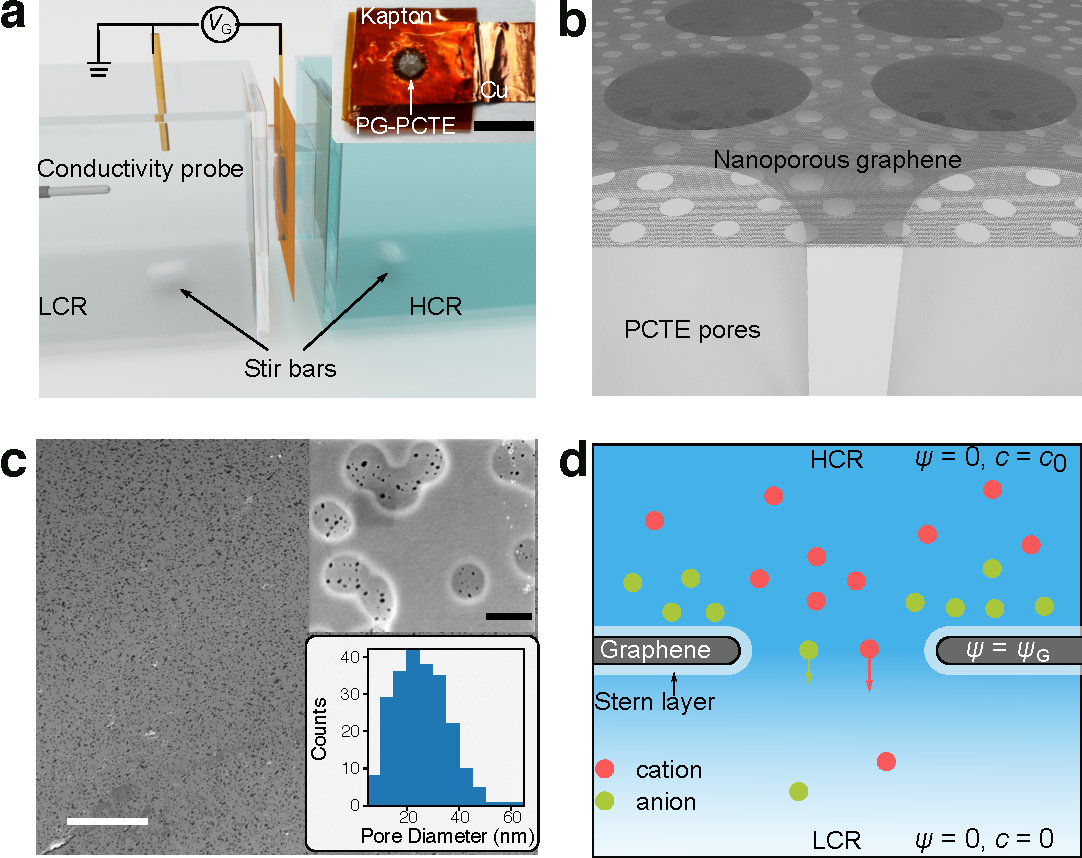
\includegraphics[width=0.85\linewidth]{img/fig1.pdf}
  \caption{a}
  \label{fig:1}
\end{figure}

\begin{figure}[htbp]
  \centering
  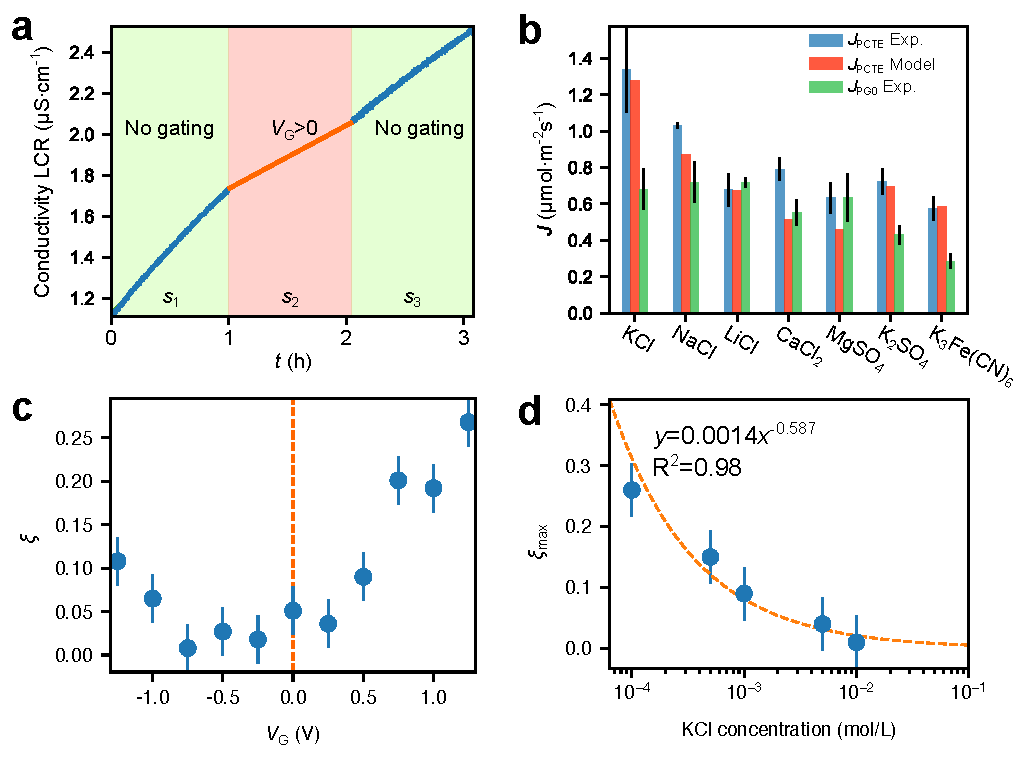
\includegraphics[width=0.85\linewidth]{img/fig2.pdf}
  \caption{a}
  \label{fig:2}
\end{figure}

\begin{figure}[htbp]
  \centering
  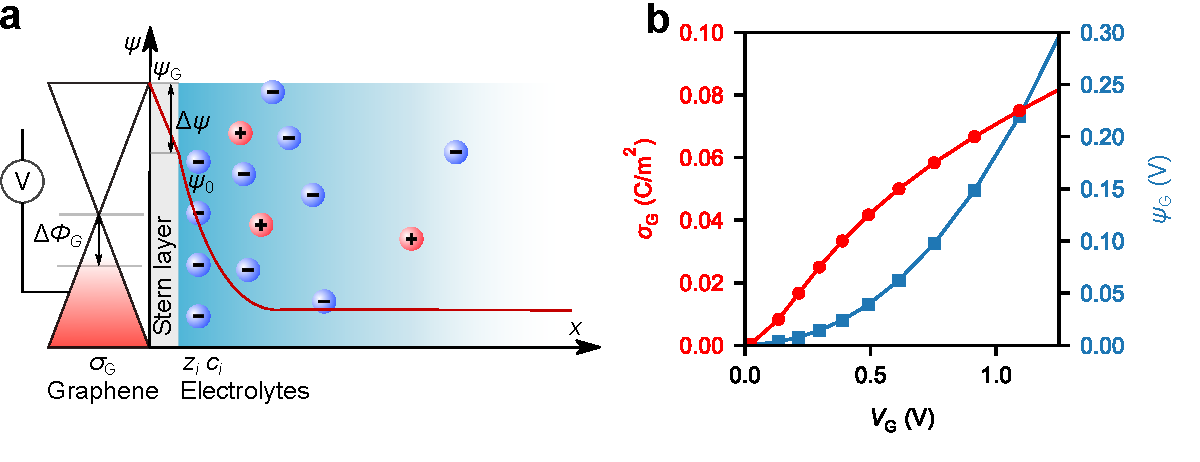
\includegraphics[width=0.95\linewidth]{img/fig3.pdf}
  \caption{a}
  \label{fig:3}
\end{figure}

\begin{figure}[htbp]
  \centering
  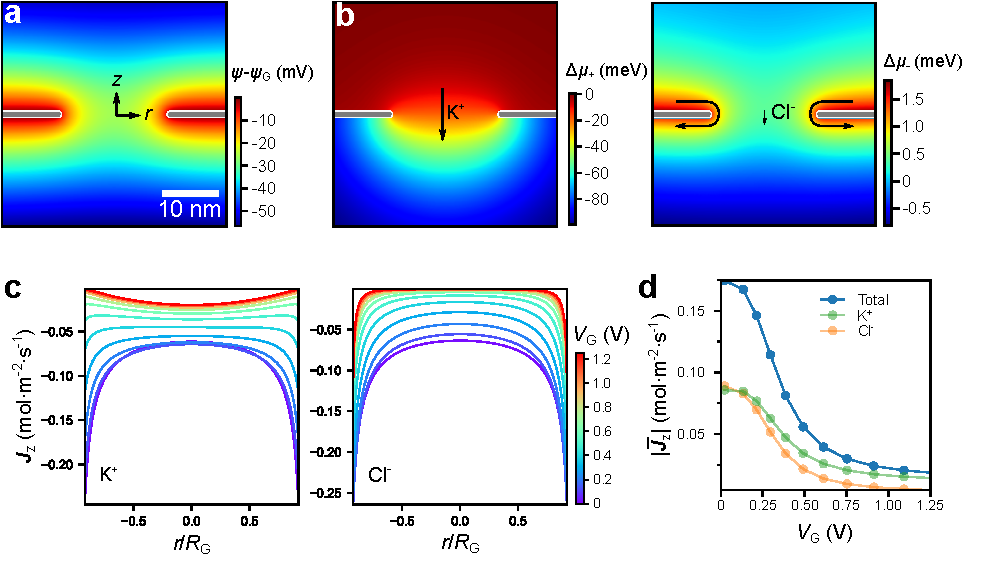
\includegraphics[width=0.85\linewidth]{img/fig4.pdf}
  \caption{a}
  \label{fig:4}
\end{figure}

\begin{figure}[htbp]
  \centering
  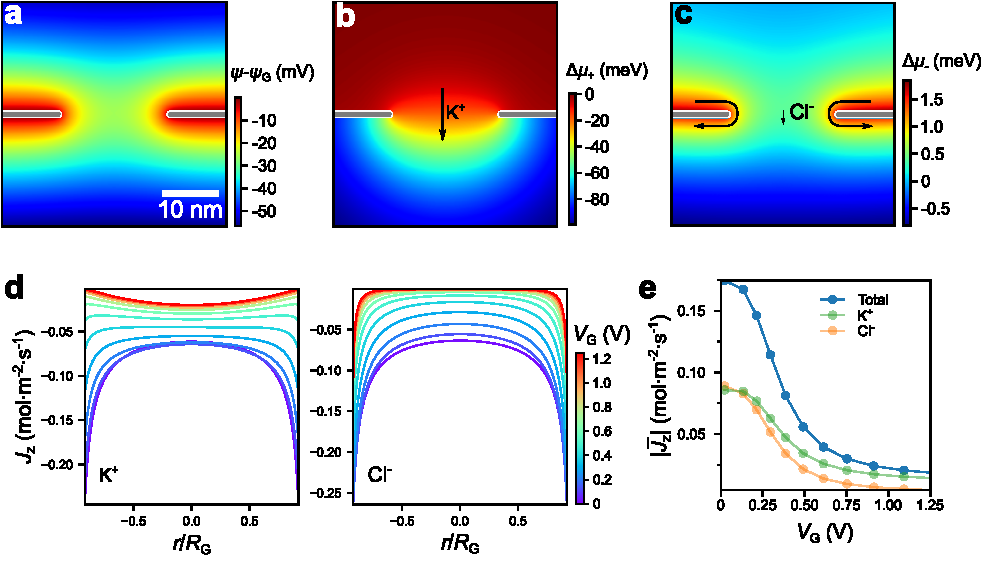
\includegraphics[width=0.9\linewidth]{img/fig5.pdf}
  \caption{a}
  \label{fig:5}
\end{figure}

\begin{figure}[htbp]
  \centering
  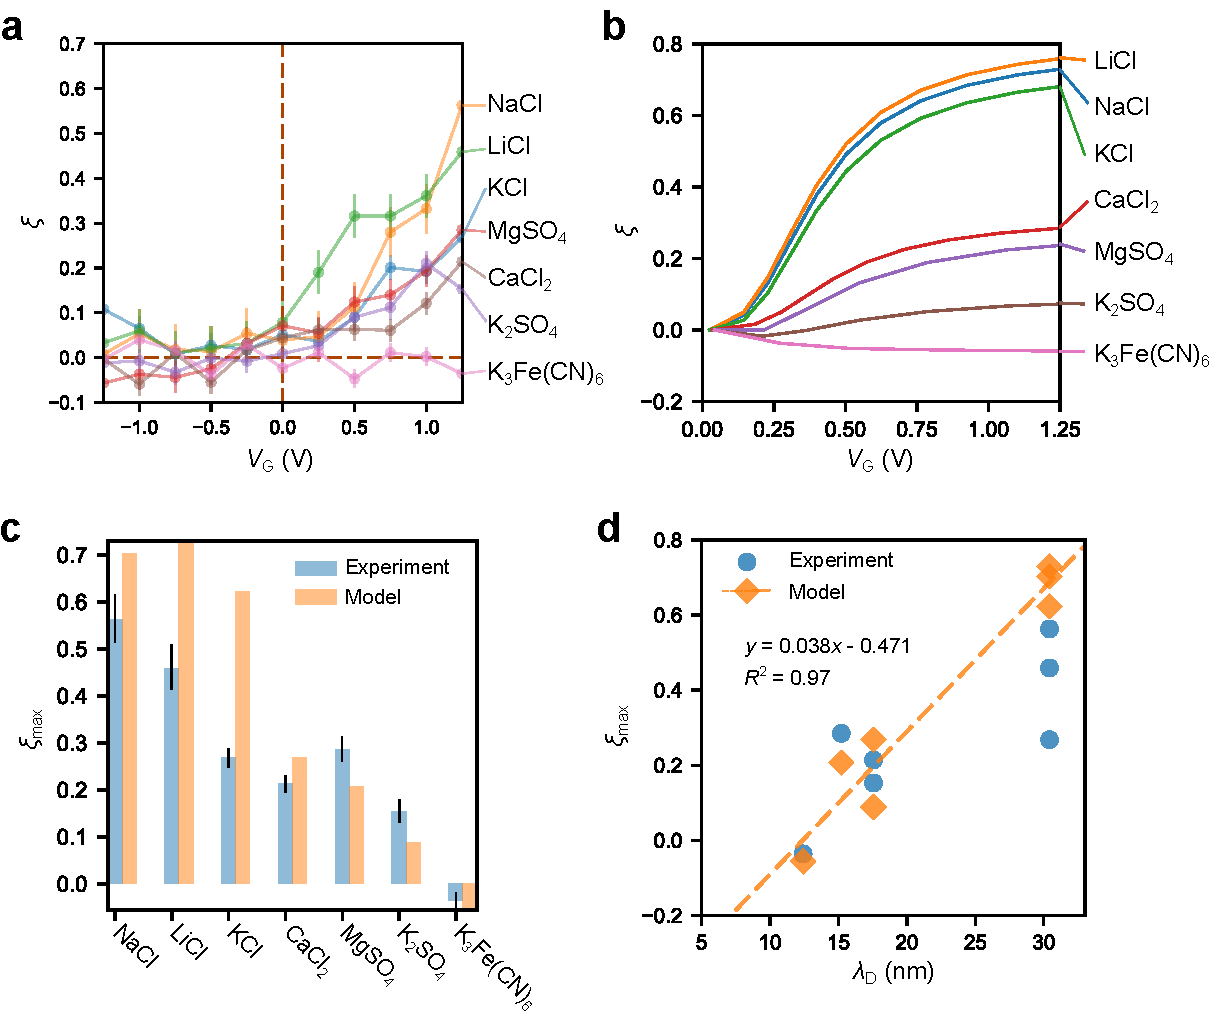
\includegraphics[width=0.9\linewidth]{img/fig6.pdf}
  \caption{a}
  \label{fig:6}
\end{figure}

\end{document}
